% igs2ejournalguide.tex
% v4.00 3-sept-2015

\NeedsTeXFormat{LaTeX2e}

% check that the math fits the two-column format:
 \documentclass[twocolumn,letterpaper]{igs}

% but use this version when submitting your article:
 %\documentclass[review,oneside]{igs}


  \usepackage{igsnatbib}
\usepackage{lmodern}
\usepackage{amsmath,amssymb,amsthm}
\usepackage{wrapfig}
\usepackage{enumitem}
\usepackage{multirow}
\usepackage{tabularx}
\usepackage{booktabs}
\usepackage{lscape}
\usepackage{color}
\usepackage{graphicx}
\usepackage{subcaption}


\definecolor{M}{rgb}{ 0,    0.4470,    0.7410}
\definecolor{MT}{rgb}{0.8500,    0.3250,    0.0980}
\definecolor{C}{rgb}{0.9290,    0.6940,    0.1250}
\definecolor{H}{rgb}{ 0.4940,    0.1840,    0.5560}
\definecolor{HC}{rgb}{0.4660 ,   0.6740 ,   0.1880}
\definecolor{R}{rgb}{0.3010 ,   0.7450 ,   0.9330}

 


\begin{document}

\title[Optimal snow-survey design for estimating winter balance]{Optimal snow-survey design for the estimation of winter balance on alpine glaciers}

\author[Pulwicki and Flowers]{Alexandra PULWICKI,$^a$
  Gwenn E. FLOWERS,$^b$}

\affiliation{%
$^a$ Department of Earth Sciences, Simon Fraser University, 8888 University Drive, Burnaby, BC, V5A 1S6, Canada\\
  $<$apulwick@sfu.ca$>$\\
 $^b$ Department of Earth Sciences, Simon Fraser University, 8888 University Drive, Burnaby, BC, V5A 1S6, Canada\\
  $<$gflowers@sfu.ca$>$ }

%%%%%%%%%%%%%%%%%%%%%%%%%%%%%%%%%
%	ABSTRACT
%%%%%%%%%%%%%%%%%%%%%%%%%%%%%%%%%

\abstract{Efficient collection of snow depth and density data is critical to a successful snow measurement campaign and to accurately estimate glacier winter balance. Extensive, high resolution and accurate snow accumulation measurements on glaciers are almost impossible to achieve so surveys need to optimize the extent and spacing of snow measurements to obtain reliable estimates of winter balance. To address this need, we estimate winter balance and root mean squared error (RMSE) using synthetic and real data from subsets of extensive surveys on three glaciers in the St. Elias Mountains, Yukon. We generate six different survey designs, which encompass possible snow sampling patterns and various numbers of measurement locations. We then use linear regression with topographic parameters to interpolate measurements. Analysis of both synthetic and real data indicates that an `midline \& transect' and`hourglass' sampling patterns result in the most efficient and accurate estimate of winter balance, while the midline pattern results in poor estimates of winter balance for all glaciers. RMSE decreases with increased sample size, with no further reduction after about 30 measurement locations. This study highlights the ability for future winter balance and snow survey studies to optimize snow data collection within a glacierized basin.

\vspace{0.3cm} Keywords: {\normalfont glacier; alpine; snow survey design; optimize; St. Elias Mountains; snow probing}}

\maketitle

%%%%%%%%%%%%%%%%%%%%%%%%%%%%%%%%%
%	INTRODUCTION
%%%%%%%%%%%%%%%%%%%%%%%%%%%%%%%%%
\section{Introduction}

\begin{figure*}
	\centering
	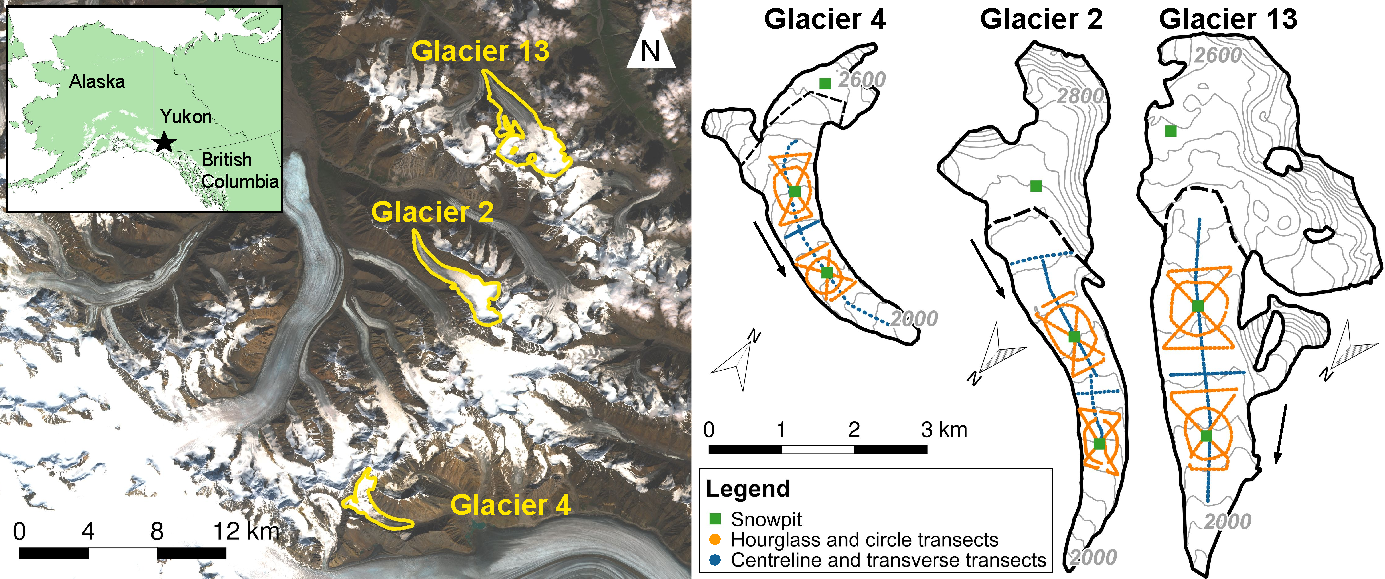
\includegraphics[width =\textwidth]{Pulwicki_Fig1.pdf}\\
	\caption{Study area location and sampling patterns for Glaciers 4, 2 and 13. (Left) Study region in the Donjek Range of the St. Elias Mountains of Yukon, Canada (inset). Imagery from Landsat8 (29 August 2013, data available from the U.S. Geological Survey). (Right) Details of the spatial sampling patterns, with midline and transverse profiles (blue dots), hourglass with inscribed circle designs (orange dots) and locations of snow-density measurements (green squares). Arrows indicate ice-flow directions. Approximate location of ELA on each glacier is shown as a black dashed line. Contour interval is 50\,m (grey).}
	\label{fig:Sampling}
\end{figure*} 

Estimates of basin-wide seasonal snow accumulation are critical for monitoring glacier mass balance and for predicting the availability and timing of surface runoff, especially in mountainous regions. The net accumulation of snow on a glacier over a winter season is known as the winter surface mass balance, or ``winter balance'' (WB) and is typically reported in meters of water equivalent (m\,w.e.) \citep{Cogley2011}. Winter balance accounts for half of the seasonally resolved mass balance, initializes ablation conditions and affects energy and mass exchange between the land and atmosphere \citep[e.g.][]{Hock2005, Reveillet2016}. 

Optimal survey designs for snow depth  are central to accurately estimating snow distribution and mass balance from \textit{in situ} measurements. Measuring snow depth and travelling between measurement locations is both time consuming and can disturb the snow, so care must be taken to choose a survey design that avoids bias, allows for the greatest variability to be measured and minimizes distance travelled \citep[e.g.][]{Shea2010,Kinar2015}. Moreover, the period of seasonal maximum snow depth can be brief, further motivating the need for time-efficient survey designs. 

% HERE'S WHAT I'M THINKING FOR DICTION:
% survey design: the whole thing: spatial sampling pattern plus # measurements
% sampling pattern: just the spatial design 
% sample size: # measurements

There are a number of different spatial sampling patterns that have been employed to obtain point measurements of snow depth, including pure random \citep[e.g.][]{Elder1991}, linear random \cite[e.g.][]{Shea2010}, nested \citep[e.g.][]{Schweizer2008}, gridded random \citep[e.g.][]{Bellaire2008, Elder2009, Bellaire2011} and gridded \citep[e.g.][]{Molotch2005a, Kronholm2007, Lopez2011}. Sampling schemes that incorporate randomness are favourable because they limit sampling bias by varying sample spacing and direction. However, they are less efficient than designs that incorporate grids. Grid-based designs minimize travel distance but measurements are biased by regularly spaced intervals and linear orientations which can result in an under-representation of  snow-depth variability \citep{Kronholm2007}.

Snow surveys on glaciers are conducted to estimate winter balance, and multi-year sampling programs are often established to monitor changes in winter balance with time. An optimized survey design requires (1) a sampling scheme that captures spatial variability and minimizes travel distance and (2) knowledge of the minimum number of measurement locations needed to estimate WB to the desired precision.  Optimization of winter-balance survey design is rarely investigated because the locations of snow-depth measurements are often dictated by field resources and logistics. 
Few studies have investigated the number of measurement locations needed to effectively sample the winter-balance distribution \citep[c.f.][]{Fountain1999,Walmsley2015}. The sampling patterns used for most winter-balance programs do not include randomness, and measurements are typically made along the glacier centreline \citep[e.g.][]{Kaser2002} to capture expected orographic effects \citep[e.g.][]{Grunewald2014}. However, centreline surveys are known to underestimate winter balance, so transverse profiles are often added to improve the reliability of the sampling scheme \citep[e.g.][]{Walmsley2015}. An hourglass with an inscribed circle (personal communication from C. Parr, 2016) is an alternative sampling scheme that captures changes in winter balance with elevation while avoiding the centreline bias, and is easy to travel. To our knowledge, no study has yet compared the performance of these different sampling patterns in estimating the spatially distributed winter balance.

% CORRECT IF WRONG. I'M THINKING THE SYNTHETIC DATA COMPARISON ADDRESSES PRECISION OF GLACIER-WIDE WB, WHILE THE REAL-DATA COMPARISON ADDRESSES ACCURACY AT REAL MEASUREMENT LOCATIONS. I THINK IT'S USEFUL TO ESTABLISH IN THE INTRO THESE TWO ELEMENTS OF THE STUDY AND USE THE WORDS THAT WILL HELP READERS CONNECT OBJECTIVES WITH RESULTS AND FIGURES.

The goal of this work is to determine the optimal survey design for estimating distributed and glacier-wide (integrated) winter balance. We consider both the spatial sampling scheme and the number of measurement locations in defining the optimal survey design. For three alpine glaciers in the St. Elias Mountains of Yukon, Canada, we explore the effects of survey design on: 
(1) the accuracy of estimated glacier-wide (integrated) winter balance in tests with synthetic data, and  
(2) the accuracy of estimated winter balance at distributed locations across the glacier by comparisons with real data. 


%%%%%%%%%%%%%%%%%%%%%%%%%%%%%%%%%
%	STUDY SITE
%%%%%%%%%%%%%%%%%%%%%%%%%%%%%%%%%

\section{Study site}

We investigate winter-balance survey design for three unnamed glaciers in the Donjek Range of southwest Yukon, Canada. Situated on the northern flanks of the St. Elias Mountains, which rise sharply from the Pacific Ocean, the Donjek Range experiences a continental climate. Monitoring of snow distribution and glacier mass balance in the St. Elias Mountains began in the 1950s and 1960s with a series of research programs, including Project ``Snow Cornice''  and the Icefield Ranges Research Project \citep{Wood1948, Danby2003}. More recent studies have focused on studies of individual alpine glaciers \citep[e.g.][]{Clarke2014,Flowers2014} as well as regional glacier mass balance and dynamics \citep[e.g.][]{Arendt2008, Burgess2013,Waechter2015}. 

Glacier 4, Glacier 2 and Glacier 13 (labelling adopted from \cite{Crompton2016}) are small alpine glaciers (3.8--12.6\,km$^2$) with simple geometries. The elevation of these glaciers ranges from 1900 to 3100\,m\,a.s.l. and ELAs are located at $\sim$2500\,m. The glaciers are generally oriented southeast-northwest in steep-walled valleys. We suspect that all three glaciers are polythermal, based on a targeted study of Glacier 2 \citep{Wilson2013} and related theoretical modelling \citep{Wilson2013a}. A detailed analysis of winter-balance estimation on these three glaciers is presented by \cite{Pulwicki2017}.


%%%%%%%%%%%%%%%%%%%%%%%%%%%%%%%%%
%	METHODS
%%%%%%%%%%%%%%%%%%%%%%%%%%%%%%%%%

\section{Methods}

Below we outline the process of determining point-scale and grid-scale values of winter balance from snow depth and density measurements. We then describe the production of gridded synthetic distributions of winter balance for each of the three study glaciers, from which synthetic sample datasets can be extracted. Finally, we present our strategy for evaluating survey design with real and synthetic data, using specific performance metrics. 

\subsection{Field measurements}

Point-scale values of winter balance are obtained from direct measurements of snow depth and density (Figure \ref{fig:Sampling}). Snow depth was measured using  3.2\,m graduated aluminium avalanche probes. 
Measurement locations followed linear and curvilinear transects in various spatial patterns termed ``midline-'' and ``transverse profiles'' and ``hourglass with inscribed circle''. 
Midline profiles, alone or combined with transverse profiles, comprise the most common survey designs used in winter-balance studies \citep[e.g.][]{Kaser2002, Machguth2006}. The midline profile aims to capture changes in winter balance with elevation, while transverse profiles provide some characterization of lateral variations in winter balance. The hourglass with inscribed circle allows for sampling in multiple directions and easy travel (personal communication from C. Parr, 2016). 

Sampling patterns were similar between study glaciers, with a sample spacing of 10--60\,m dictated by protocols for safe glacier travel. Each observer made 3--4 individual depth measurements within $\sim$1\,m at each survey location. Snow-depth measurements were largely restricted to the ablation area, where the clear distinction between snow and ice ensures that only snow from the most recent accumulation season is measured. In total, we collected more than 9000 snow-depth measurements throughout the study area. Snowpit-density profiles were measured using a wedge cutter and spring scale at three locations on each glacier that were distributed in elevation. A mean density was then calculated for each glacier and used to convert snow depth at all measurement locations to values of point-scale winter balance. The mean density and standard deviation was 348$\pm$13\,kg\,m$^{-3}$ on Glacier 4, 333$\pm$26\,kg\,m$^{-3}$ on Glacier 2 and 349$\pm$38\,kg\,m$^{-3}$ on Glacier 13. All point-scale values of winter balance located within a common digital elevation model (DEM) gridcell ($40\times40$\,m) were averaged to obtain a single value of winter balance in each sampled gridcell. 

\subsection{Tests with synthetic data}

A synthetic glacier-wide distribution of winter balance is obtained for each study glacier by linear regression of the gridcell-averaged values of WB (obtained as described above) on topographic parameters derived from a SPIRIT SPOT-5 DEM \citep{Korona2009}. These parameters include commonly used quantities \citep[e.g.][]{McGrath2015} such as elevation, slope, aspect, distance from glacier centreline, ``northness'', curvature and a wind redistribution parameter. The regression is used, along with cross-validation and Bayesian model averaging, to obtain a set of regression coefficients for each glacier  \citep{Pulwicki2017}. The resulting distribution of winter balance, hereafter referred to as the ``synthetic distribution of winter balance'' is determined by multiplying fitted regression coefficients by the corresponding topographic parameters for each gridcell in the DEM. We use the regression as an emulator to generate realistic winter-balance distributions that we can treat as synthetic data. 

Synthetic data are used to evaluate survey design, including the sampling pattern and sample number. 
We investigate various survey designs that are unique combinations of six different sampling patterns: midline, midline and transverse profiles, circle, hourglass, hourglass with inscribed circle and random. The random pattern is restricted to the area encompassed by the original field measurements (Figure \ref{fig:Sampling}). 
%[I WOULD INCLUDE THIS SENTENCE BECAUSE WE HAVE TO JUSTIFY WHY WE DIDN'T USE THE WHOLE GLACIER] All sampling patterns are restricted to the ablation area, where terrain is accessible and measurements of snow depth are generally unambiguous. 
For each sampling pattern we investigate the effect of sample size $n$, where $n$ ranges from a minimum of eight (constrained by the use of seven topographic parameters in the interpolation) to a maximum determined by the number of gridcells sampled by a given pattern (ranging from 57 to 228). 

To generate a synthetic sample size $n$ for a given sampling pattern (e.g. hourglass), we extract values of winter balance from the glacier-wide synthetic distribution 
that are regularly spaced within the chosen sampling pattern. The geographic locations of the patterns are fixed based on the original field measurements.    
We then add low or high noise to the synthetic sample set. Low noise is defined by a normal distribution with zero mean and a standard deviation derived from a series of high-density subgrid-scale measurements of winter balance on each glacier \citep{Pulwicki2017}.  
High noise is defined in the same way, but with the standard deviation three times that of low noise. This value is approximately equal to that derived by \citet{Pulwicki2017} to represent multiple sources of uncertainty including subgrid-scale variability (as in the low-noise case), the assignment of snow density in the conversion of snow depth to winter balance and measurement interpolation.
For each synthetic sample of winter balance, a randomly chosen value from the high- or low-noise distribution is added to the sample value.

To assess the performance of a given survey design (sampling pattern and sample size), we compare the original synthetic distribution of winter balance to that obtained when the topographic regression is performed using only the noisy synthetic sample set. 
%[WE ARE ACTUALLY ONLY COMPARING INTEGRATED VALUES - SHOULD MENTION THIS SOMEWHERE] -> WE COMPARE BOTH INTEGRATED (COLOURFUL GRAPH) AND DISTRIBUTED (PURPLE MAP FIGURE)
Since the noise is sampled randomly from a distribution, we repeat the regression to create 100 realizations of ``estimated winter balance'' from which we can calculate a mean and standard deviation. Comparison of the ``synthetic'' and ``estimated'' winter balances allows us to assess both the accuracy (using the mean estimated winter balance) and the precision (using the standard deviation of the estimated winter balances) 
%[NOT QUITE] 
of a given survey design, with the caveat that the utility of the results is limited by the extent to which the simulated distribution represents a plausible reality.   
 
 \subsection{Tests with real data}
 
 Using real data offers an opportunity to evaluate survey design in a different way, and provides a check on the result obtained in the synthetic tests. Here we aim to test how well the estimated winter balance compares with field measurements as a function of sampling pattern and sample number. In this series of tests, we extract subsets of $n$ samples of the observed winter balance (as described in ``Field measurements'') from individual sampling patterns (e.g. hourglass with inscribed circle) and use each subset of observed values to generate an ``estimated winter balance'' with a linear regression as described above. Because these values are real data, they already contain noise. Instead of adding noise, as in the synthetic case, we repeat the regression 100 times with randomly selected subsets of $n$ values; this approach means the values will not be regularly spaced. From these 100 realizations we calculate a mean and standard deviation of the estimated winter balance. We then compute the RMSE between all observed values of winter balance and the co-located estimates of winter balance. This comparison allows us to assess both the accuracy and precision [NOT QUITE] of a given survey design in predicting real data, but is limited to the locations of the original field measurements. By its nature, this comparison also combines the performance of the survey design with the performance of the regression. 
 %[TRUE?]  -> yes but we are comparing it to the RMSE of the regression with full data. So even on G4, where the regression is poor, we have good convergence. But I guess we're just comparing a bad regression with low n to a bad regression with high n...

 \subsection{Performance metrics}
 
To quantify the performance of each survey design, we use two metrics. The first metric we term ``convergence'', defined as the sample size ($n_{\rm c}$) needed to obtain a mean estimated glacier-wide winter balance within 5\% of the target value in the synthetic tests, or RMSE $\leq$5\% in the comparison with real data. To determine $n_{\rm c}$ we smooth the mean estimated values of glacier-wide winter balance as a function of $n$ to avoid spurious results arising from the random nature of adding noise to the synthetic samples or selecting the subset of observed values.
Convergence is a metric that describes the minimum number of measurement locations required to produce an accurate (within 5\%) estimate of winter balance. The second metric we term ``variability'', defined as the sample size ($n_{\rm v}$) needed to obtain a standard deviation of the estimated glacier-wide winter balance within 25\% of the target value in the synthetic tests, or RMSE $\leq$25\% in the comparison with real data. We again smooth the standard deviation of estimated values of glacier-wide winter balance as a function of $n$, in order to determine $n_{\rm v}$. 
``Variability'' is a metric that describes the sensitivity of the estimated winter balance to noise in the synthetic tests and sampling locations in the comparisons with real data.
%[I WANTED TO SAY IT QUANTIFIED PRECISION, BUT IT DOESN'T BECAUSE WE COMPARE THE STD WITH THE ``TRUE'' VALUE] -> the metric is still a measure of the "width" of the colour bar, it's just that the threshold width changes for each glacier
We also compute the total travel distance required to obtain the measurements required for a given survey design. An efficient survey will have low values of  $n_{\rm c}$ and $n_{\rm v}$ as well as a short travel distance. 

%%%%%%%%%%%%%%%%%%%%%%%%%%%%%%%%%%%%%%%%%%%
%%  RESULTS
%%%%%%%%%%%%%%%%%%%%%%%%%%%%%%%%%%%%%%%%%%%
\section{Results }

\subsection{Tests with synthetic data}

\begin{figure*}
	\centering
	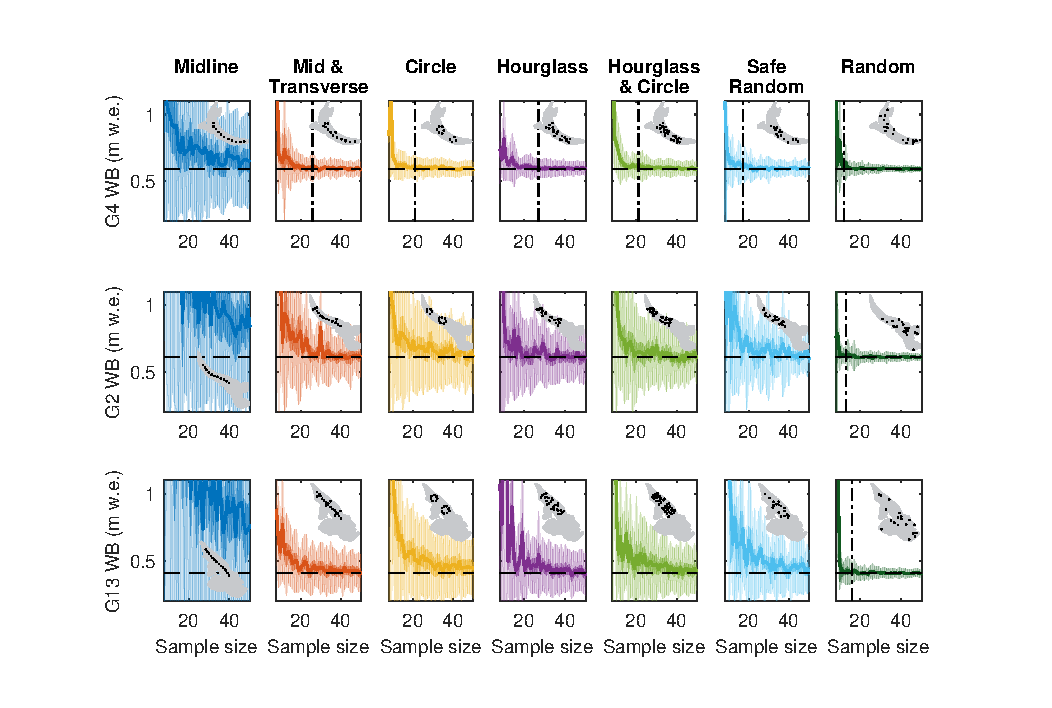
\includegraphics[width =\textwidth]{SyntheticObsWB.pdf}\\
	\caption{Glacier-wide winter balance (WB) estimated with various sampling patterns (columns) and sample sizes (x-axes) for Glacier 4 (top row), Glacier 2 (middle row) and Glacier 13 (bottom row). Insets show example sampling patterns. Bold solid lines are smoothed mean values of WB estimated from 100 linear regressions of synthetic samples of WB on topographic parameters for each spatial sampling patterns (columns) and sample sizes from 8 to $>$45 (x-axes). Dark and light shading indicate the standard deviation in estimated WB for low- and high-noise cases, respectively. Horizontal dashed lines indicate the synthetic target value of glacier-wide WB. Vertical dotted lines show sample size $n_{\rm c}$ that achieves an accuracy of 5\% (difference between smoothed mean and target value). Vertical dot-dashed lines show sample size $n_{\rm v}$ for which the standard deviation comes within 5\% of the target value in the high-noise case. Not all sampling patterns have $n_{\rm c}$ and $n_{\rm v}$ within the range of samples sizes shown.}
	\label{fig:SyntheticObsWB}
\end{figure*}



Based on the synthetic tests, the most effective sampling patterns are circle (C), hourglass (H) or midline \& transect (MT), depending on the metric used ($n_{\rm c}$ or $n_{\rm v}$) and the glacier (Figure \ref{fig:SyntheticObsWB}, Table \ref{tab:SynthPatternRanks}). 
With all sampling patterns, winter balance is overestimated at low sample size.
For Glacier 4, C and H converge equally quickly ($n_{\rm c}=11$) to the target synthetic value of glacier-wide winter balance, and exhibit the least sensitivity to noise ($n_{\rm v}=11$). For Glacier 13, MT is best, with $n_{\rm c}=12$ and $n_{\rm v}=36$. For Glacier 2, C and H converge most quickly ($n_{\rm c}=13$) but variability is minimized with MT ($n_{\rm v}=24$). Among these three sampling patterns, C requires the least travel and MT the most (Table \ref{tab:SynthPatternRanks}, bottom three rows). 
If using H, C, HC or MT sampling patterns, a sample size $\leq 15$ is sufficient for convergence of the mean to the target synthetic value of winter balance for all glaciers. 
To insure convergence in the presence of noise for all glaciers, a sample size of  $\leq 36$ is sufficient for MT, $ \leq 46$ for H and $\leq 52$ for HC. For C the sample size is up to 99. These values are much lower for Glaciers 4 and 2 than for Glacier 13.   
Of note is the fact that H, C and HC perform similarly as judged by convergence ($n_{\rm c}$) for all glaciers, and variability ($n_{\rm v}$) for Glacier 4; C performs much more poorly in terms of variability for Glaciers 2 and 13.

\begin{table*}[]
\centering
\caption{Synthetic data tests. Ranking of survey designs from 1 to 6 (top row) for Glaciers 4, 2 and 13 (G4, G2, G13) based on three different metrics (see text): $n_{\rm c}$ (top three rows), $n_{\rm v}$ (middle three rows) and travel distance ($d$) required to perform survey (bottom three rows). Sampling patterns are: midline (M), midline and transverse (MT), circle (C), hourglass (H), hourglass and circle (HC) and random (R). Colours follow figures. Values in parentheses are $n_{\rm c}$, $n_{\rm v}$ or travel distance (km). Travel distances given for random sampling scheme are averages.}
\label{tab:SynthPatternRanks}
\begin{tabular}{clclclclclclcl}
\hline
 Metric         && \textbf{1} && \textbf{2} && \textbf{3} && \textbf{4} && \textbf{5} && \textbf{6} \\
 \hline
                & \textbf{G4}    & \textcolor{C}{C}, \textcolor{H}{H}         & (11)         &          &         &  \textcolor{MT}{MT}, \textcolor{HC}{HC}, \textcolor{R}{R}         & (12)         &          &           &          &  & \textcolor{M}{M} & (17) \\
$n_{\rm c}$         & \textbf{G2}   & \textcolor{C}{C}, \textcolor{H}{H}         & (13)         &          &           & \textcolor{MT}{MT}, \textcolor{HC}{HC}         & (14)         &          &          & \textcolor{R}{R}         & (15) & \textcolor{M}{M} & (45) \\
                & \textbf{G13} & \textcolor{MT}{MT}         & (12)         & \textcolor{HC}{HC},\textcolor{C}{C} & (14)         &  \textcolor{H}{H}                 & (15)         &                  &           & \textcolor{R}{R}         & (16) & \textcolor{M}{M} & (104) \\
\hline
                & \textbf{G4}   & \textcolor{C}{C},  \textcolor{H}{H}         & (11)         &         &           & \textcolor{HC}{HC}         & (12)         & \textcolor{R}{R}                 & (13)         & \textcolor{MT}{MT} & (14) & \textcolor{M}{M} & (--) \\
$n_{\rm v}$         & \textbf{G2}   & \textcolor{MT}{MT}         & (24)         & \textcolor{H}{H}         & (29)         & \textcolor{HC}{HC},  \textcolor{R}{R}         & (30)        &                  &         &  \textcolor{C}{C}         & (50) & \textcolor{M}{M} & (--) \\
                & \textbf{G13} & \textcolor{MT}{MT}         & (36)         & \textcolor{H}{H}         & (46)         & \textcolor{R}{R}, \textcolor{HC}{HC}                 & (52)         &         &          & \textcolor{C}{C}         & (99) & \textcolor{M}{M} & (--) \\
\hline
                & \textbf{G4}   & \textcolor{C}{C}         & (4.8) & \textcolor{M}{M}         & (6.3) & \textcolor{H}{H}                 & (6.9)         & \textcolor{R}{R}         & ($\sim$7.9) & \textcolor{MT}{MT}         & (8.3) & \textcolor{HC}{HC} & (11.1) \\
$d$        & \textbf{G2}   & \textcolor{M}{M}         & (4.3) & \textcolor{C}{C}         & (5.7) & \textcolor{H}{H}                 & (8.4)         & \textcolor{MT}{MT} & (8.6)         & \textcolor{R}{R}                 & ($\sim$9.2) & \textcolor{HC}{HC} & (12.5) \\
                & \textbf{G13} & \textcolor{C}{C}         & (7.0) & \textcolor{M}{M}         & (8.0) & \textcolor{H}{H}                 & (10.6)         & \textcolor{MT}{MT} & (11.0)         & \textcolor{R}{R}                 & ($\sim$11.3) & \textcolor{HC}{HC} & (16.8)\\
\hline
\end{tabular}
\end{table*}


\begin{figure*}
	\centering
	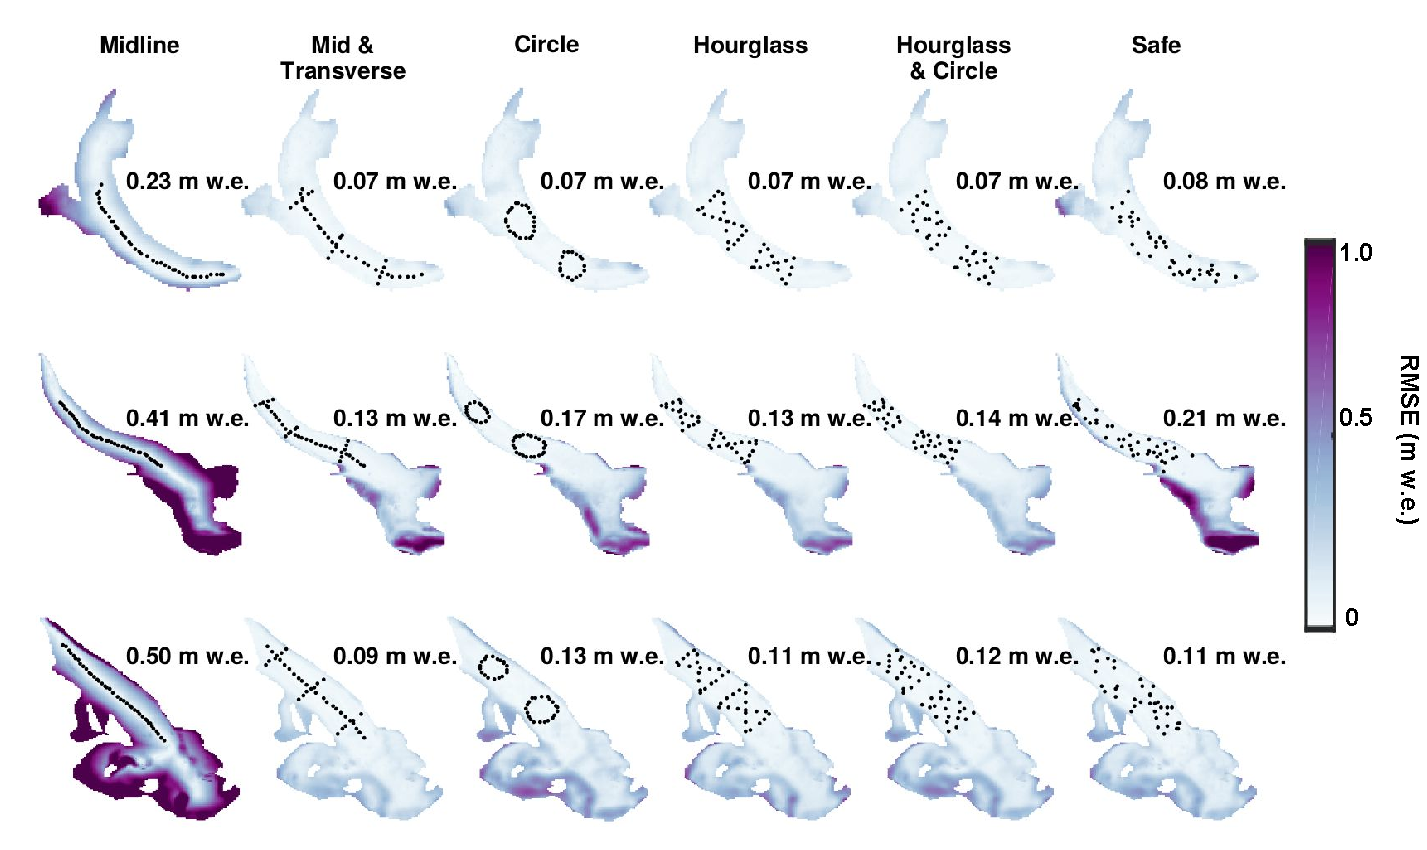
\includegraphics[width =\textwidth]{SynObsRMSEmap.pdf}\\
	\caption{RMSE between synthetic target distribution of WB and [MEAN?] WB estimated with various sample patterns, $n=40$ and 100 regressions of the high-noise sample set. Sampling patterns are shown in columns for Glacier 4 (top row), Glacier 2 (middle row) and Glacier 13 (bottom row). RMSE for the entire glacier is displayed. Synthetic sampling locations are shown as black dots.}
	\label{fig:SynObsRMSEmap}
\end{figure*}


The remaining sampling patterns, midline (M) and random (R), are less effective for estimating the synthetic winter balance, though R performs comparably to the others particularly as assessed by convergence $n_{\rm c}$. 
Midline is decisively the worst sampling pattern, ranked last for all glaciers for both $n_{\rm c}$ and $n_{\rm v}$. Winter balance estimated with a midline sampling pattern is highly sensitive to noise for all glaciers and only achieves convergence to the target synthetic value for low sample sizes ($n_{\rm c}=14$) on Glacier 4. 

Although the convergence patterns are generally similar between glaciers, the sample sizes needed to accurately estimate winter balance ($n_{\rm c}$) and insure convergence in the presence of noise ($n_{\rm v}$) are smallest for Glacier 4 and largest for Glacier 13 for all sampling patterns (compare top row to bottom row in Figure  \ref{fig:SyntheticObsWB}). The RMSE between estimated and synthetic values of winter balance is also greater on Glaciers 2 and 13 than on Glacier 4, especially in the accumulation area (Figure \ref{fig:SynObsRMSEmap}). When the midline pattern is used, the RMSE is high over a large areal fraction of the glacier.

\subsection{Tests with real data}

\begin{figure*}
	\centering
	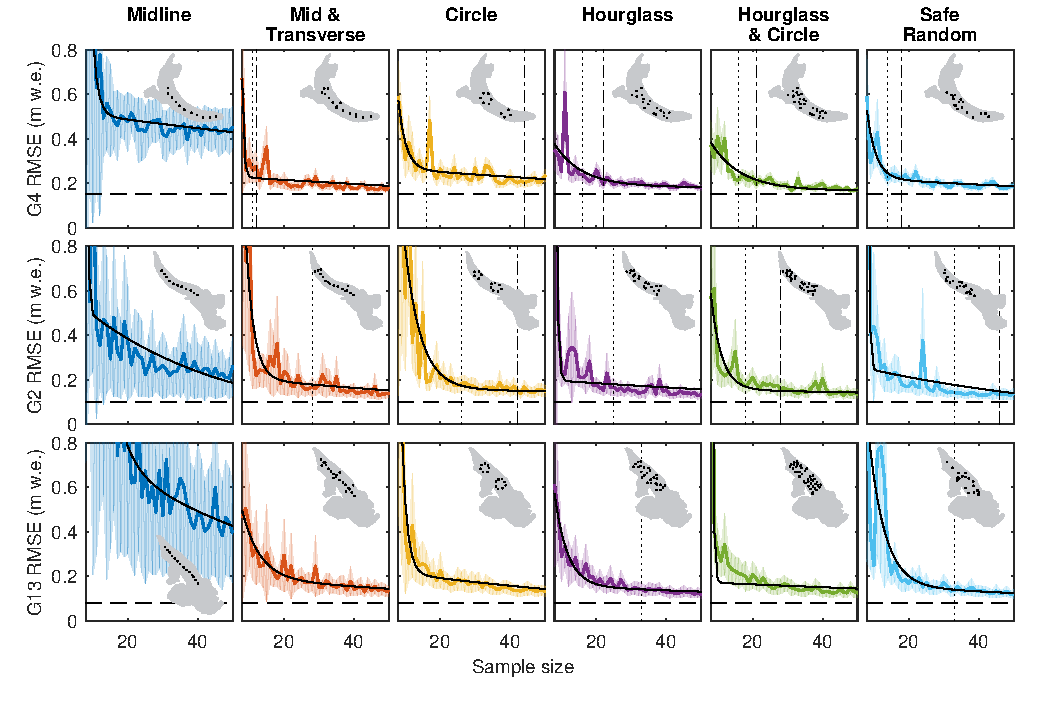
\includegraphics[width =\textwidth]{DataObsWB.pdf}\\
	\caption{RMSE between all observed values of winter balance and the co-located estimates of winter balance from randomly selected subsets of the real data, with various sampling schemes (columns) and sample sizes (x-axes) for Glacier 4 (top row), Glacier 2 (middle row) and Glacier 13 (bottom row). Insets show example sampling schemes. Bold solid lines are smoothed mean values of RMSE from 100 linear regressions. Shading indicates the standard deviation [STD OF RMSE?] arising from different subsets of the randomly chosen data. Horizontal dashed lines indicate  RMSE when all data are used to estimate WB.  Vertical dotted lines show sample size $n_{\rm c}$ that achieves RMSE $\leq 5$\% (difference between smoothed mean and target value). Vertical dot-dashed lines show sample size $n_{\rm v}$ for which the standard deviation comes within 5\% of the target value. Not all sampling patterns have $n_{\rm c}$ and $n_{\rm v}$ within the range of samples sizes shown.}
	\label{fig:RealObsWB}
\end{figure*}

%%% REAL DATA TABLE %%%%%
\begin{table*}[]
\centering
\caption{Real data tests. Ranking of survey designs from 1 to 6 (top row) for Glaciers 4, 2 and 13 (G4, G2, G13) based on two different metrics (see text): $n_{\rm c}$ (top three rows) and $n_{\rm v}$ (bottom three rows). Sampling patterns are: midline (M), midline and transverse (MT), circle (C), hourglass (H), hourglass and circle (HC) and random (R). Colours follow figures. Values in parentheses are $n_{\rm c}$ or $n_{\rm v}$. Travel distances for each sampling pattern are given in Table \ref{tab:SynthPatternRanks}.}
\label{tab:RealPatternRanks}
\begin{tabular}{clclclclclclcl}
\hline
 Metric         && \textbf{1} && \textbf{2} && \textbf{3} && \textbf{4} && \textbf{5} && \textbf{6} \\
 \hline
                & \textbf{G4}   & \textcolor{R}{R}         & (19) & \textcolor{MT}{MT}         & (22)         &  \textcolor{H}{H}        &  (24)        & \textcolor{HC}{HC}         & (25)           &  \textcolor{C}{C}        & (44) & \textcolor{M}{M} & (--) \\
$n_{\rm c}$         & \textbf{G2}   & \textcolor{H}{H}         & (16)         &  \textcolor{HC}{HC}        &  (17)          & \textcolor{MT}{MT}, \textcolor{C}{C}        & (20)         &          &          & \textcolor{R}{R}         & (21) & \textcolor{M}{M} & (29) \\
                & \textbf{G13} & \textcolor{R}{R}         & (16)         & \textcolor{HC}{HC} & (19)         & \textcolor{C}{C}                 & (20)         &           \textcolor{H}{H}        &   (21)        & \textcolor{MT}{MT}         & (36) & \textcolor{M}{M} & (--) \\
\hline
                & \textbf{G4}   & \textcolor{R}{R}         & (21)         &   \textcolor{MT}{MT}        &  (22)         & \textcolor{C}{C}         & (25)         & \textcolor{H}{H}                 & (26)         & \textcolor{HC}{HC} & (29) & \textcolor{M}{M} & (47) \\
$n_{\rm v}$         & \textbf{G2}   & \textcolor{H}{H}         & (22)         & \textcolor{HC}{HC}, \textcolor{C}{C}         & (25)         &            &         &  \textcolor{R}{R}                & (26)        &  \textcolor{MT}{MT}         & (28) & \textcolor{M}{M} & (38) \\
                & \textbf{G13} & \textcolor{R}{R}         & (20)         & \textcolor{HC}{HC}         & (29)         & \textcolor{C}{C}                 & (30)         &  \textcolor{H}{H}        & (34)         & \textcolor{MT}{MT}         & (47) & \textcolor{M}{M} & (--) \\
%\hline
%                & \textbf{G4}   & \textcolor{C}{C}         & (4.8) & \textcolor{M}{M}         & (6.3) & \textcolor{H}{H}                 & (6.9)         & \textcolor{R}{R}         & ($\sim$7.9) & \textcolor{MT}{MT}         & (8.3) & \textcolor{HC}{HC} & (11.1) \\
%$d$        & \textbf{G2}   & \textcolor{M}{M}         & (4.3) & \textcolor{C}{C}         & (5.7) & \textcolor{H}{H}                 & (8.4)         & \textcolor{MT}{MT} & (8.6)         & \textcolor{R}{R}                 & ($\sim$9.2) & \textcolor{HC}{HC} & (12.5) \\
%                & \textbf{G13} & \textcolor{C}{C}         & (7.0) & \textcolor{M}{M}         & (8.0) & \textcolor{H}{H}                 & (10.6)         & \textcolor{MT}{MT} & (11.0)         & \textcolor{R}{R}                 & ($\sim$11.3) & \textcolor{HC}{HC} & (16.8)\\
\hline
\end{tabular}
\end{table*}

%[I WONDER IF THIS IS REALLY NOT A FAIR TEST, USING THE RANDOM SAMPLE OF REAL DATA, RATHER THAN REGULARLY SPACED. HOW EASY IS IT TO GENERATE THE CURVES FOR THE REGULARLY SPACED CASE?] -> see email

The RMSE between estimated and observed winter balance decreases rapidly with increasing sample size for most sampling patterns on any of the glaciers (Figure \ref{fig:RealObsWB}), with inflection points around $n=10$. 
The performance of the sampling patterns as assessed by comparison with real data (Table \ref{tab:RealPatternRanks}) shows hourglass (H) to rank highest for Glacier 2, and random (R) to rank highest for Glaciers 4 and 13, for both $n_{\rm c}$ and $n_{\rm v}$. Hourglass \& circle (HC), circle (C) and midline \& transverse (MT) rank anywhere from 2--5, while midline (M) is again last in every case. 
Compared to the tests with synthetic data, greater sample sizes are generally required to reach the 5\% targets [NOT A FAIR COMPARISON SINCE RMSE AND WB ARE TWO DIFF QUANTITIES?], but the range of $n_{\rm c}$ and $n_{\rm v}$ are smaller  [AGAIN PROB NOT FAIR BECAUSE RANDOMNESS ARISES FROM DIFF SOURCES IN REAL VS SYNTH TESTS].
None of the sampling patterns result in RMSE falling to that of the full dataset with $n < 45$, but R comes close for Glaciers 4 and 13, while H comes closest for Glacier 2. A sample size of $n \leq 30$ is sufficient to reach the $n_{\rm c}$ and $n_{\rm v}$ targets for all sampling patterns excluding the midline. 
Though the rankings in Table \ref{tab:RealPatternRanks} differ from those using synthetic data (Table \ref{tab:SynthPatternRanks}), the overall picture of performance is not dissimilar in that midline (M) is the only pattern that can be easily ruled out for all glaciers based on either $n_{\rm c}$ or $n_{\rm v}$.      

%%%%%%%%%%%%%%%%%%%%%%%%%%%%%%%%%%%%%%%%%%%
%% DISCUSSION
%%%%%%%%%%%%%%%%%%%%%%%%%%%%%%%%%%%%%%%%%%%
\section{Discussion}

The optimal survey design for our study region is the midline \& transverse or hourglass pattern with a sample size of $\sim30$. Based on both synthetic and real data, both designs result in low error, are least sensitive to noise and involve relatively short travel distance. A sample size greater than 30 does not significantly improve the accuracy of WB estimated and does not decrease error. This surprisingly low number of measurement locations indicates that high-resolution sampling is not required to accurately estimate WB. Instead, taking measurements throughout the study basin should be prioritized when choosing a survey design. If the goal is to estimate WB then field resources should be more strongly allocated to distributing measurement locations to capture basin-scale spatial trends in WB since error is greatest in areas far from sampling locations and in areas with extreme values of topographic parameters. Based on our results, midline is a poor choice of sample design regardless of the number of measurement locations. In contrast, \citep{Surjanovic2016} finds that a midline pattern does well for some ablation survey designs and \cite{Fountain1999} found that as few as 5 stakes are needed to estimate mass balance of a glacier. We hypothesize that a greater number of measurement locations are needed to estimate winter balance because snow distribution is governed by processes that vary on shorter spatial scales than processes that govern ablation. \cite{Walmsley2015} recommends one measurement for every 50\,m elevation band, which would amount to 9--12 measurement locations on our study glaciers when only the ablation area is considered (17--24 for the full glacier). This suggestion is consistent with the $n_{\rm c}$ or $n_{\rm v}$ value for circle, hourglass and midline \& transect on some of the glaciers. 

The most effective survey designs capture the dominant WB-elevation trend but also have measurement locations in gridcells that span the range of other topographic parameters. Despite the fact that the synthetic distribution of WB on Glaciers 2 and 13 is largely controlled by elevation, measurements locations that are not along the midline are needed to constrain the regression. When the midline pattern is used, the topographic parameters (excluding elevation) fall within a narrow range so the regression becomes sensitive to noise. Further, the accuracy of estimated WB does not improve at large sample sizes along a midline pattern because the sampling locations do not capture relationships between WB and the remaining topographic parameters. However, if there are a large portion of measurement locations far from the midline then the elevation trend may be less strong resulting in larger errors. Random and hourglass \& circle patterns may have larger errors on Glaciers 2 and 13 as a result of the higher proportion of measurement locations far from the midline. 

On Glacier 4, the standard deviation of WB due to noise and the number of measurement locations needed to estimate WB is smaller than Glaciers 2 and 13. This trend is likely a result of the small influence of topographic parameters in the distribution of synthetic distribution of WB. The synthetic distribution of WB is derived from a linear regression between field measurements of WB and topographic parameters that explains little of the observed variance (R$^2=$0.07). As a result, glacier-wide WB is approximately equal to the mean of WB field measurements. This mostly uniform distribution of snow can therefore be described with few measurement locations, regardless of where the measurements are obtained. 

We find that, on average, WB is over-estimated with small sample sizes ($<20$), especially on Glaciers 2 and 13 with $n<10$. We hypothesize that over-estimation results from an exaggeration of the elevation regression coefficient, which is the dominant explanatory parameter for Glaciers 2 and 13. At small sample sizes, the elevation trend over-shadows the relationships with other topographic parameters and is sensitive to noise, which results in large WB values in the accumulation area. Our finds are inconsistent with \cite{Walmsley2015}, who found that using only midline probings underestimates WB.

Further work into the optimization of snow survey survey design is needed. The most obvious limitation of our study is the restriction of survey design to accessible locations in the ablation area. Lack of measurements in the accumulation area is a sub-optimal survey design. However, direct measurements of snow depth in the accumulation area are extremely costly because a large amount of time is needed to dig a snow pit, especially in regions with high accumulation. Given the importance of spatially distributed measurements though, there is likely an optimal balance between costly measurements in the accumulation area and less costly measurements in the ablation area. Use of more efficient snow-depth measurement methods, such a ground-penetrating radar (GPR) and lidar, in the accumulation area can also be investigated. Additional extensions to our work include an investigation of the size and placement of hourglass patterns and to optimize measurement locations based on factors such as topographic parameters. 


%%%%%%%%%%%%%%%%%%%%%%%%%%%%%%%%%%
% CONCLUSION
%%%%%%%%%%%%%%%%%%%%%%%%%%%%%%%%%%
\section{Conclusion}

From an analysis of synthetic and real WB data, we find that `midline \& transect' and`hourglass' sampling patterns with a sample size of approximately 30 measurement locations is the optimal survey design for estimating glacier-wide WB. Since a relatively low sample size is needed and errors are greatest in the accumulation area, we recommend that field resources be allocated such that measurements locations are distributed throughout the sample basin rather than obtaining high-resolution WB measurements. A midline sampling pattern results in poor estimates of WB and high sensitivity to noise. We find that WB is over-estimated with very small sample sizes ($n<10$) and along the midline so care should be made to adequately sample the basin to capture changes in elevation as well as transverse variation in WB. 

\section{Acknowledgements}

We thank the Kluane First Nation (KFN), Parks Canada and the Yukon Territorial Government for granting us permission to work in KFN Traditional Territory and Kluane National Park and Reserve. We are grateful for financial support provided by the Natural Sciences and Engineering Research Council of Canada, Simon Fraser University (including the KEY Big Data Initiative) and the Northern Scientific Training Program. We kindly acknowledge Kluane Lake Research Station, Sian Williams, Lance Goodwin and Trans North pilot Dion Parker for facilitating field logistics. We are grateful to Alison Criscitiello and Coline Ariagno for all aspects of field assistance and Sarah Furney for assistance with data entry. Thank you to Etienne Berthier for providing us with the SPIRIT SPOT-5 DEM and for assistance in DEM correction. We are grateful to Derek Bingham and Michael Grosskopf for assistance with statistics. Laura Thomson, Leif Anderson, Dave Bigelow and Erik Young all provided thoughtful and constructive comments on drafts of the manuscript.


%----------------------------------------------------------------------------------------
%	REFERENCE LIST
%----------------------------------------------------------------------------------------
%
%\bibliography{MastersLit.bib}
%\bibliography{/home/glaciology1/Documents/MastersDocuments/MastersLit}
\bibliography{/Users/Alexandra/Documents/SFU/MastersDocuments/MastersLit}
\bibliographystyle{igs}

%----------------------------------------------------------------------------------------

\end{document}
